\documentclass[11pt]{article}
\fontfamily{Arial}
\usepackage{graphicx} %necessario per l'inserimento delle immagini
%opening
\title{Progetto Basi di Dati}
\author{Baesso Nicola, Egidi Annalisa}

\begin{document} %inizia il documento vero e proprio

\maketitle %crea il titolo
\begin{center} %mette il contenuto in centro
	%
\includegraphics{../logo.jpeg}	
\end{center}

\section{Abstract}
La Scuola di Musica Il Pentagramma è un’associazione culturale senza fini di lucro che dal 1982 ha lo scopo di promuovere, diffondere e sviluppare la conoscenza, l’apprendimento ed il perfezionamento della musica moderna e classica in tutte le sue tecniche strumentali e canore.\\
L'associazione organizza corsi, senza limiti di età, per l'apprendimento di tecniche strumentali o vocali, di registrazione, composizione e di tutto ciò che sia collegato alla musica. Inoltre promuove la creazione di gruppi musicali e organizza eventi e concerti in proprio o in accordo con locali o enti privati e locali, in modo da diffondere la cultura musicale sia ai suoi associati sia a chiunque voglia partecipare, e quindi contribuire alla diffusione di tale cultura.\\
I corsi, suddivisi tra corsi individuali, musica d'insieme, teatro e corsi propedeutici, sono tenuti da docenti diplomati al conservatorio e alcuni sono svolti anche dagli stessi dirigenti della scuola. Hanno durata di 30,45 o 60 minuti a seconda della tipologia del corso. I corsi individuali offrono inoltre dei momenti di controllo, in cui gli allievi mostrano i loro progressi ad una giuria interna, e per chi ambisce ad un percorso professionale l'associazione prevede una suddivisione in livelli, accessibili tramite il superamento di un apposito esame che ne certifica le qualità acquisite nel percorso.\\
L'associazione vuole costruire una base di dati affinché possa organizzare al meglio le attività dell'associazione, oltre che mantenere uno storico delle attività passate e dei membri che ne hanno fatto parte nel corso del tempo.

\section{Analisi dei requisiti}
	Si vuole rappresentare, attraverso una basi di dati, le attività e gli eventi organizzati dall'associazione Il Pentagramma.\\\\
	Ogni \textbf{persona} collegata all'associazione è caratterizzata da codice fiscale, nome, cognome, data di nascita, numero di telefono e indirizzo email. Una persona può essere un associato, un docente, un dirigente oppure uno studente.\\\\
	Di un \textbf{associato} è rilevante il codice della tessera a lui associata, la data d'iscrizione all'associazione e la data di scadenza dell'iscrizione.\\\\
	Per un \textbf{docente} si vuole sapere la specializzazione in cui si è diplomato, la data di conseguimento del diploma, la data d'inizio dell'attività di insegnamento e, nel caso il docente non insegni più nella scuola, la data di fine. Inoltre, in caso di insegnamento in più corsi, è rilevante conoscere, assieme al corso, la data di inizio e l'eventuale fine di docenza in quel corso. Per un \textbf{dirigente}, che è anche un docente, è rilevante conoscere l'unico ruolo che copre all'interno dell'associazione, la data di inizio in quel ruolo e, se presente, la data di fine in quel ruolo (che può combaciare con la data di fine insegnamento).\\\\
	Uno \textbf{studente} è caratterizzato dalla tipologia (amatoriale o professionale) di percorso che segue e, in caso di percorso professionale, il livello a cui lo studente stesso si trova. Inoltre è d'interesse sapere la data d'inizio delle lezioni e l'eventuale data di fine. Infine, se lo studente risulta iscritto all'associazione ma frequenta dei corsi diversi rispetto ai corsi con cui ha cominciato, è rilevante conoscere la data d'inizio e di eventuale fine di frequentazione di ciascun corso frequentato.\\\\
	Un \textbf{corso} è caratterizzato dal nome, dalla durata (in minuti) di una lezione e dal numero d'incontri in un mese. Un corso può essere individuale o collettivo.Per i corsi collettivi è d'interesse avere anche una descrizione breve del corso stesso. Tale attributo non è rilevante per i corsi individuali in quanto già esplicativi col nome stesso.\\\\
	Una \textbf{sede} è caratterizzata da nome, città e via nella quale si trova. Una sede può essere usata come sede per le lezioni o come sede per gli eventi. Per una \textbf{sede per eventi} è rilevante conoscere anche il numero massimo di posti disponibili.\\\\
	Un \textbf{evento} è caratterizzato da nome, genere, sede dove viene svolto e numero di spettatori, essendo aperti al pubblico. Se l'evento non è direttamente organizzato dall'associazione, oppure l'associazione non è l'unica organizzatrice dell'evento, allora è d'interesse anche conoscere il nome degli organizzatori o co-organizzatori. Inoltre è d'interesse conoscere i brani svolti durante l'evento, oltre agli studenti che li eseguono, se partecipanti. Negli eventi sono compresi anche i \textbf{saggi}, organizzati solo dall'associazione e dove partecipano solo gli studenti della scuola.\\\\
	Un \textbf{brano} è caratterizzato da nome, artista e genere. Ai fini delle attività dell'associazione, non sono d'interesse altre informazioni relative ai brani e ai relativi artisti.\\\\
	Un \textbf{esame} è caratterizzato dallo studente che lo effettua, la data in cui è stato fatto, il livello per cui è valido l'esame, l'esito dell'esame (passato o non passato) e la commissione, composta da al più 3 docenti. Per l'associazione non è rilevante conoscere i docenti esterni presenti nelle commissioni, sono d'interesse solo i docenti interni. Per una \textbf{audizione} sono d'interesse gli stessi campi meno il livello, essendo la stessa da effettuare anche per gli allievi che seguono un percorso amatoriale, e l'esito.
	\subsection{Glossario dei termini}
		\begin{tabular}{|c|c|c|c|}
			\hline
			Termine & Descrizione & Sinonimi & Collegamenti\\
			\hline
			Persona & Persona che interagisce & Associato, Docente,&$\emptyset$\\
			& con l'associazione & Dirigente, Studente &\\
			\hline
			Associato & Persona iscritta all'associazione & Persona &$\emptyset$ \\
			\hline
			Docente & Docente di musica dell'associazione  & Persona & Dirigente\\
			\hline
			& Persona incaricata agli aspetti & & \\
			Dirigente & organizzativi dell'associazione & Persona, Docente &$\emptyset$ \\
			 & e garante degli obiettivi programmatici && \\
			\hline
			Studente & Persona che beneficia & Persona & $\emptyset$\\
			& delle lezioni musicali & & \\
			\hline
			Corso & Servizio offerto dall'associazione al quale, & &\\
			& iscrivendosi, si diventa&$\emptyset$ &$\emptyset$\\
			& studenti & &\\
			\hline
			Sede & Luogo per lo svolgimento &$\emptyset$ &$\emptyset$\\
			& dei servizi offerti & &\\
			\hline
			& Spettacolo rivolto ad un pubblico.& &\\
			Evento & Può essere organizzato &$\emptyset$ &$\emptyset$\\
			& dall'associazione stessa o & &\\
			& in collaborazione con enti esterni. & &\\
			\hline
			& Evento organizzato& &\\
			& esclusivamente dall'associazione& &\\
			Saggio& che permette agli studenti di mettere& Evento &$\emptyset$\\
			&  alla prova le conoscenze & &\\
			&  acquisite nei corsi scelti & &\\
			\hline
			Brano & Spartito studiato ed &$\emptyset$ &$\emptyset$\\
			& eseguito da uno studente & &\\
			\hline
			Esame & Test che lo studente svolge &$\emptyset$ &$\emptyset$\\
			& per il passaggio ad un livello superiore & &\\
			\hline
			& Momento di valutazione& &\\
			Audizione & obbligatorio per gli studenti&$\emptyset$ & Esame\\
			& dell'associazione & &\\
			\hline
			\end{tabular}
	\subsection{Operazioni tipiche}
		Le seguenti operazioni vengono generalmente effettuate a cadenza mensile.\\\\
		\begin{tabular}{|c|c|}
			\hline
			1) Inserimento e lettura studenti nei corsi scelti & 100 al mese\\
			\hline
			2) Controllo delle iscrizioni relative ai soci & 30 al mese\\
			\hline
			3) Inserimento di eventi & 10 al mese\\
			\hline
		\end{tabular}
		\\\\
		Mentre le seguenti operazioni vengono effettuate durante l'anno.\\\\
		\begin{tabular}{|c|c|}
			\hline
			4) Archiviazione dell'anno accademico con cadenza trimestrale& 5 all'anno\\
			\hline
			5) Controllo dei docenti e dei dirigenti & 60 all'anno\\
			\hline
			6) Controllo delle sedi & 80 all'anno\\
			\hline
			7) Controllo dei corsi & 350 all'anno\\
			\hline
			8) Controllo ed eventuale scrittura del numero di spettatori negli eventi & 50 all'anno\\
			\hline
		\end{tabular}
\section{Progettazione concettuale}
	\subsection{Lista delle entità}
		\begin{tabular}{|c|c|c|}
			\hline
			\multicolumn{3}{|c|}{\textbf{Persona}: colui/colei che interagisce con l'associazione}\\
			\hline
			\underline{CF} & char(16) primary key & Il Codice Fiscale della persona\\
			\hline
			Nome & varchar(30) & Il nome della persona\\
			\hline
			Cognome & varchar(30) & Il cognome della persona\\
			\hline
			DataNascita & date & La data di nascita della persona\\
			\hline
			Contatto &  & I contatti della persona, si divide in\\
			&  &\textbf{Telefono} e \textbf{Email}.\\
			Telefono & char(10) & Il numero di telefono della persona\\
			Email & varchar(50) & L' indirizzo mail della persona\\
			\hline
		\end{tabular}
		\\\\ \textbf{Persona} si specializza in \textbf{Associato}, \textbf{Studente} e \textbf{Docente}.\\\\
		\begin{tabular}{|c|c|c|}
			\hline
			\multicolumn{3}{|c|}{\textbf{Associato}: un iscritto all'associazione}\\
			\hline
			\underline{CodiceTessera} & char(10) primary key & Il codice della tessera associata all'associato\\
			\hline
			DataIscrizione & date & La data in cui l'associato risulta iscritto\\
			\hline
			DataScadenza & date & La data di scadenza dell'iscrizione\\
			\hline
		\end{tabular}
		\\\\\\
		\begin{tabular}{|c|c|c|}
			\hline
			\multicolumn{3}{|c|}{\textbf{Studente}: colui che frequenta i corsi organizzati dall'associazione}\\
			\hline
			Tipologia & char(1) & La tipologia del corso frequentato,\\
			 &  & si distingue tra amatoriale(A) o professionale(P) \\
			\hline
			Livello (0,1) & char(2) & Il livello in cui si posiziona lo studente\\
			\hline
			&  & Il periodo in cui lo studente frequenta\\
			PeriodoLezioni &  & o ha frequentato i corsi dell'associazione, si divide in\\
			&  &\textbf{InizioLezioni} e \textbf{FineLezioni}.\\
			InizioLezioni & date & La data d'inizio di frequenza dei corsi\\
			FineLezioni (0,1) & date & La data di fine di frequenza dei corsi\\
			\hline
		\end{tabular}
		\\\\\\
		\begin{tabular}{|c|c|c|}
			\hline
			\multicolumn{3}{|c|}{\textbf{Docente}: una persona che insegna nei corsi dell'associazione}\\
			\hline
			Diploma & varchar(30) & Il diploma in possesso\\
			\hline
			DataDiploma & date & La data di acquisizione del diploma\\
			\hline
			&  & Periodo in cui il docente insegna o ha insegnato\\
			PeriodoDocenza &  & per conto dell'associazione, si divide in\\
			&  &\textbf{InizioDocenza} e \textbf{FineDocenza}.\\
			InizioDocenza & date & Data d'inizio dell'attività d'insegnamento\\
			FineDocenza (0,1) & date & Data di fine dell'attività d'insegnamento\\
			\hline
		\end{tabular}
		\\\\
		\textbf{Docente} può specializzarsi in \textbf{Dirigente}
		\\\\
		\begin{tabular}{|c|c|c|}
			\hline
			\multicolumn{3}{|c|}{\textbf{Dirigente}: docente con un ruolo di rilevanza nell'organizzazione dell'associazione}\\
			\hline
			Ruolo & varchar(30) & Il ruolo ricoperto all'interno dell'associazione\\
			\hline
			&  & Periodo in cui il dirigente ha coperto un determinato\\
			PeriodoDirigenza &  & ruolo all'interno dell'associazione, si divide in\\
			&  &\textbf{InizioDirigenza} e \textbf{FineDirigenza}.\\
			InizioDirigenza & date & Data d'inizio in cui si è ricoperto il ruolo\\
			FineDirigenza (0,1) & date & Data di fine del ruolo ricoperto\\
			\hline
		\end{tabular}
		\\\\\\
		\begin{tabular}{|c|c|c|}
			\hline
			\multicolumn{3}{|c|}{\textbf{Attività}: attività didattica organizzata dall'associazione}\\
			\hline
			InizioAttivita & date & La data d'inizio dell'attività\\
			\hline
			FineAttivita (0,1) & date & La data di fine dell'attività\\
			\hline
		\end{tabular}
		\\\\\\
		\begin{tabular}{|c|c|c|}
			\hline
			\multicolumn{3}{|c|}{\textbf{Corso}: percorso didattico offerto dall'associazione}\\
			\hline
			\underline{NomeCorso} & varchar(30) primary key & Il nome del corso\\
			\hline
			DurataLezione & int & La durata della singola lezione, in minuti\\
			\hline
			LezioneMese & int & Il numero di lezioni mensili che il corso prevede\\
			\hline
		\end{tabular}
		\\\\ \textbf{Corso} si specializza in \textbf{Individuale} e \textbf{Collettivo}.\\\\
		\begin{tabular}{|c|c|c|}
			\hline
			\multicolumn{3}{|c|}{\textbf{Individuale}: corso che offre lezioni individuali}\\
			\hline
		\end{tabular}
		\\\\
		\begin{tabular}{|c|c|c|}
			\hline
			\multicolumn{3}{|c|}{\textbf{Collettivo}: corso con lezioni in cui più studenti partecipano contemporaneamente}\\
			\hline
			Descrizione & varchar(50) & Breve descrizione sul corso\\
			\hline
		\end{tabular}
		\\\\\\
		\begin{tabular}{|c|c|c|}
			\hline
			\multicolumn{3}{|c|}{\textbf{Sede}: luogo dove le attività e gli eventi dell'associazione sono tenuti}\\
			\hline
			\underline{NomeSede} & varchar(50) primary key & Il nome della sede\\
			\hline
			Locazione &  & Le indicazioni dove si trova una sede, si divide in\\
			&  &\textbf{Citta} e \textbf{Indirizzo}.\\
			Citta & varchar(30) & La città dove si trova la sede\\
			Indirizzo & varchar(50) & L'indirizzo della sede\\
			\hline
		\end{tabular}
		\\\\ \textbf{Sede} si specializza in \textbf{SedeLezione} e \textbf{Sedevento}.\\\\
		\begin{tabular}{|c|c|c|}
			\hline
			\multicolumn{3}{|c|}{\textbf{SedeLezione}: luogo indicato per usufruire dei corsi dell'associazione}\\
			\hline
		\end{tabular}
		\\\\
		\begin{tabular}{|c|c|c|}
			\hline
			\multicolumn{3}{|c|}{\textbf{Sedevento}: luogo indicato per gli eventi in cui l'associazione è coinvolta}\\
			\hline
			MaxPosti & int & La capienza relativa alla sede\\
			\hline
		\end{tabular}
		\\\\\\
		\begin{tabular}{|c|c|c|}
			\hline
			\multicolumn{3}{|c|}{\textbf{Evento}: manifestazione in cui è coinvolta l'associazione}\\
			\hline
			\underline{NomeEvento} & varchar(50) & Il nome dell'evento\\
			\hline
			NumSpettatori & int & Gli spettatori che hanno partecipato\\
			\hline
			GenereEvento & varchar(20) & Il genere del'evento\\
			\hline
			Organizzazione &  & Chi ha organizzato l'evento, si divide in\\
			&  &\textbf{Organizzatore} e \textbf{Co-Organizzatore}.\\
			Organizzatore (0,1) & varchar(50) & Elenco di enti che hanno organizzato\\
			& & l'evento di cui l'associazione fa da promoter\\
			Co-Organizzatore (0,1) & varchar(50) & Elenco di enti che hanno organizzato \\
			& & l'evento assieme all'associazione\\
			\hline
		\end{tabular}
		\\\\
		\textbf{Evento} può specializzarsi in \textbf{Saggio}
		\\\\
		\begin{tabular}{|c|c|c|}
			\hline
			\multicolumn{3}{|c|}{\textbf{Saggio}: manifestazione organizzata dall'associazione dove si esibiscono gli allievi della stessa}\\
			\hline
		\end{tabular}
		\\\\
		\begin{tabular}{|c|c|c|}
			\hline
			\multicolumn{3}{|c|}{\textbf{Scaletta}: elenco di brani eseguiti da vari allievi in determinati eventi}\\
			\hline
		\end{tabular}
		\\\\\\
		\begin{tabular}{|c|c|c|}
			\hline
			\multicolumn{3}{|c|}{\textbf{Brano}: canzone suonata negli eventi dagli allievi}\\
			\hline
			\underline{NomeBrano} & varchar(50) primary key & Il nome del brano\\
			\hline
			\underline{Artista} & varchar(50) primary key & Il nome dell'artista di un brano\\
			\hline
			GenereBrano & varchar(20) & Il genere del brano\\
			\hline
		\end{tabular}
		\\\\\\
		\begin{tabular}{|c|c|c|}
			\hline
			\multicolumn{3}{|c|}{\textbf{Esame}: verifica per il passaggio di livello di un allievo}\\
			\hline
			\underline{LivelloAbilitazione} & char(2) primary key & Il livello a cui l'esame è indirizzato\\
			\hline
			\underline{DataEsame} & date primary key & La data in cui l'esame è stato sostenuto\\
			\hline
		\end{tabular}
		\\\\\\
		\begin{tabular}{|c|c|c|}
			\hline
			\multicolumn{3}{|c|}{\textbf{Audizione}: verifica del progresso di un allievo}\\
			\hline
			\underline{DataAudizione} & date primary key & La data in cui l'audizione è stata sostenuta\\
			\hline
		\end{tabular}
	\subsection{Lista delle relazioni}
		Studente-Audizione: \textbf{Allievo}\\
		-Uno studente partecipa ad almeno una audizione (1,N)\\
		-Un audizione deve essere svolta da almeno uno studente (1,N)\\
		\\
		Docente-Audizione: \textbf{Auditore}\\
		-Un docente deve essere presente ad almeno una audizione (1,N)\\
		-Un audizione deve essere presente almeno un docente (1,N)\\
		\\
		Studente-Esame: \textbf{Esaminato}\\
		-Un studente può partecipare a uno o più esami (0,N)\\
		-Ad ogni esame partecipa almeno uno studente (1,N)\\
		\begin{tabular}{|c|c|c|}
			\hline
			\multicolumn{3}{|c|}{Attributi di \textbf{Esaminato}}\\
			\hline
			EsitoEsame & bool & L'esito dell'esame\\
			\hline
		\end{tabular}
		\\\\
		Docente-Esame: \textbf{Esaminatore}\\
		-Un docente può prendere parte a uno o più esami (0,N)\\
		-Ogni esame ha almeno un docente (1,N)\\
		\\
		Studente-Scaletta: \textbf{Performance}\\
		-Uno studente può essere inserito in una o più scalette (0,N)\\
		-Una scaletta è composta da almeno uno studente (1,N)\\
		\\
		Studente-Attivita: \textbf{Apprendimento}\\
		-Uno studente è coinvolto in almeno un'attività (1,N)\\
		-Ogni attività ha almeno uno studente (1,N)\\
		\\
		Docente-Attivita: \textbf{Insegnamento}\\
		-Ogni attività è tenuta da un docente (1,1)\\
		-Ogni docente prende parte ad almeno un'attività (1,N)\\
		\\
		Brano-Scaletta: \textbf{BranoEseguito}\\
		-Ogni scaletta ha almeno un brano (1,N)\\
		-Ogni brano è presente in almeno una scaletta (1,N)\\
		\\
		Attivita-SedeLezione: \textbf{LuogoLezione}\\
		-Un'attività viene svolta in una sede per le lezioni (1,1)\\
		-Ogni sede per le lezioni ospita almeno un'attività (1,N)\\
		\\
		Attivita-Corso: \textbf{Erogazione}\\
		-Un'attività è legata ad un solo corso (1,1)\\
		-Un corso è legato ad almeno un'attività (1,N)\\
		\\
		Scaletta-Evento: \textbf{Esecuzione}\\
		-Ogni scaletta si riferisce ad un evento (1,1)\\
		-Ogni evento ha una scaletta (1,1)\\
		\\
		Evento-Sedevento: \textbf{LuogoEvento}\\
		-Ogni evento è tenuto in una sede per eventi (1,1)\\
		-Ogni sede per eventi ospita almeno un evento (1,N)\\
	\subsection{Schema ER}
		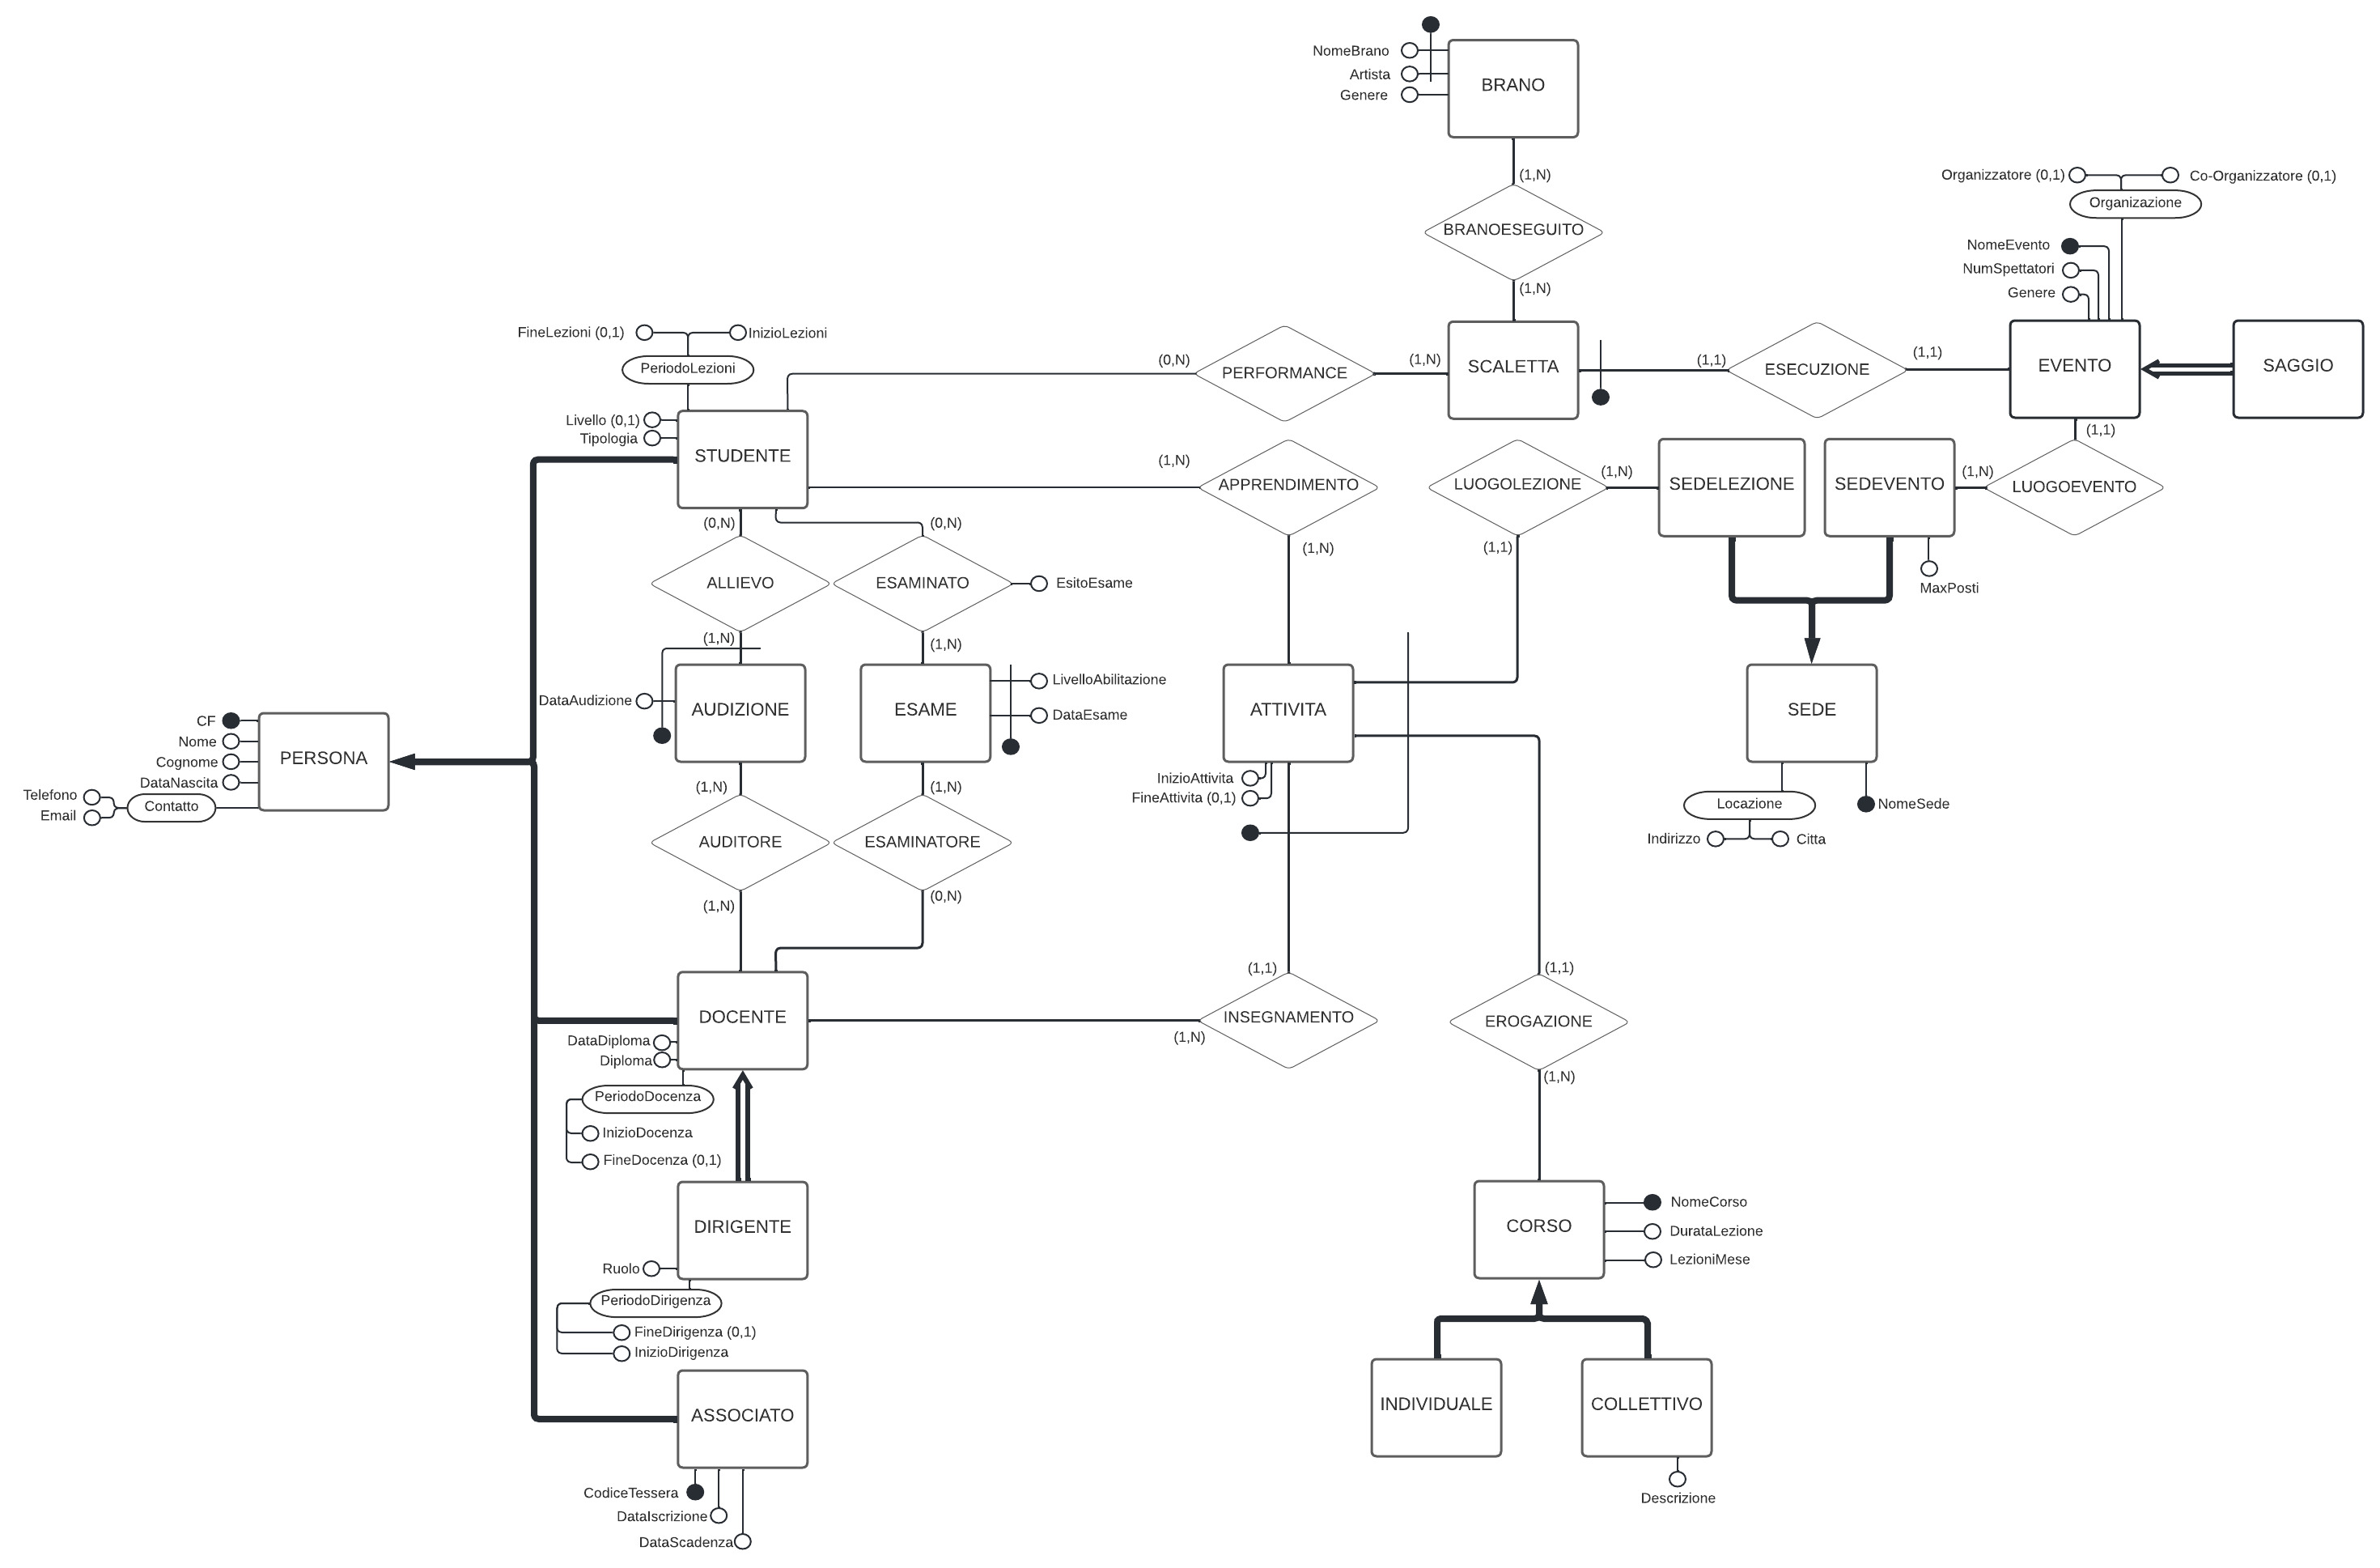
\includegraphics[scale=0.6]{../SchemaConcettuale/ER-LUCIDCHART - ER-concettuale 1.jpeg}
	\subsection{Vincoli non esprimibili nello Schema ER}
		Auditore:\\ -Per ogni studente, tra gli auditori dev'essere presente il docente con cui frequenta il corso.\\\\ Docente:\\ -FineDocenza, se presente, deve avere un valore superiore rispetto a InizioDocenza.\\\\ Studente:\\ -FineLezioni, se presente, deve avere un valore superiore rispetto a InizioLezioni.\\\\ Dirigente:\\ -FineDirigenza, se presente, deve avere un valore superiore rispetto a InizioDirigenza.\\ -Un dirigente non può ricoprire lo stesso ruolo più volte.\\\\ Associato:\\ -DataScadenza dev'essere successiva a DataIscrizione.\\\\ Esaminato:\\ -lo studente deve avere la tipologia "professionale".\\\\ Esaminatore:\\ -ogni esame ha al più 3 docenti.\\\\ Attivita:\\ -FineAttività, se presente, deve avere un valore superiore rispetto a InizioAttività.\\\\ Corso:\\ -durataLezione deve avere un valore inferiore a 60.\\\\ Evento:\\ -Organizzatore e Co-organizzatore si escludono a vicenda, ovvero se Organizzatore è non nullo, Co-Organizzatore è nullo e viceversa.\\\\ Saggio:\\ -Organizzatore e Co-organizzatore sono nulli.
\section{Progettazione logica}
	\subsection{Eliminazione delle generalizzazioni}
		Per le varie generalizzazioni, si è scelto di seguire percorsi differenti. Di seguito i dettagli:\\
		-\textbf{Persona}: si è scelto di sostituire la generazione con più relazioni. La corporazione degli attributi delle entità figlia nell'entità genitore porterebbe a tuple molto grandi e con un numero di valori nulli non indifferente, oltre ad una inevitabile complicazione della gestione. D'altro canto, inglobare gli attributi dell'entità genitore nelle entità figlie porterebbe a seri problemi di ridondanze e inconsistenze. Si è quindi ritenuto più opportuno collegare le varie entità figlie all'entità genitore tramite delle relazioni, in modo da escludere ogni possibile ridondanza e inconsistenza, mantenendo anche delle tuple senza eccessivi valori nulli.\\
		-\textbf{Docente}: per questa generalizzazione parziale si è scelto di accorpare l'entità figlia nella madre. Poichè il numero di tuple riguardanti i dirigenti è al più uguale al numero di tuple riguardanti i docenti, l'avere più tuple con valori nulli non risulta invadente. Quindi un docente viene riconosciuto anche come dirigente se almeno gli attributi RuoloDirigente e InizioDirigenza sono non nulli, altrimenti viene riconosciuto solo come docente.\\
		-\textbf{Corso}: si è scelto anche in questo caso di accorpare le entità figlie nell'entità madre, essendoci solo un attributo differente tra le varie entità. I corsi sono distinti tramite il nuovo attributo TipologiaCorso, e la descrizione deve essere non nulla solo se il corso è di tipo collettivo.\\
		-\textbf{Sede}: anche per questa generalizzazione totale si è scelto di accorpare le entità figlie nell'entità genitore, essendoci pure in questo caso solo un attributo differente tra le varie entità. Per distinguere tra le due tipologie di sedi si utilizza l'attributo Utilizzo. Ciò impone anche il controllo su MaxPosti, che deve essere non nullo solo se la sede è utilizzata per gli eventi.\\
		-\textbf{Evento}: si è scelto di accorpare l'entità figlia nell'entità genitore figlia poichè l'entità figlia non porta alcuna ulteriore informazione. Per distinguere un evento da un saggio si utilizza l'attributo TipoEvento. Inoltre è necessario che, in caso l'evento sia un saggio, sia Organizzatore che Co-Organizzatore devono essere entrambi nulli.\\
	\subsection{Analisi delle ridondanze}
		L'attributo "NumeroStudenti" nella entità "Attivita" è ridondante in quanto si può ricavare tramite la relazione "Apprendimento".
		Tale ridondanza affligge l'operazione n°1:
		
		Op.1: Inserimento e lettura studenti nei corsi scelti.
	\subsection{Partizionamento / Accorpamento di entità e associazioni}
	\subsection{Scelta degli identificatori principali}
	\subsection{Diagramma E-R ristruttutato}
		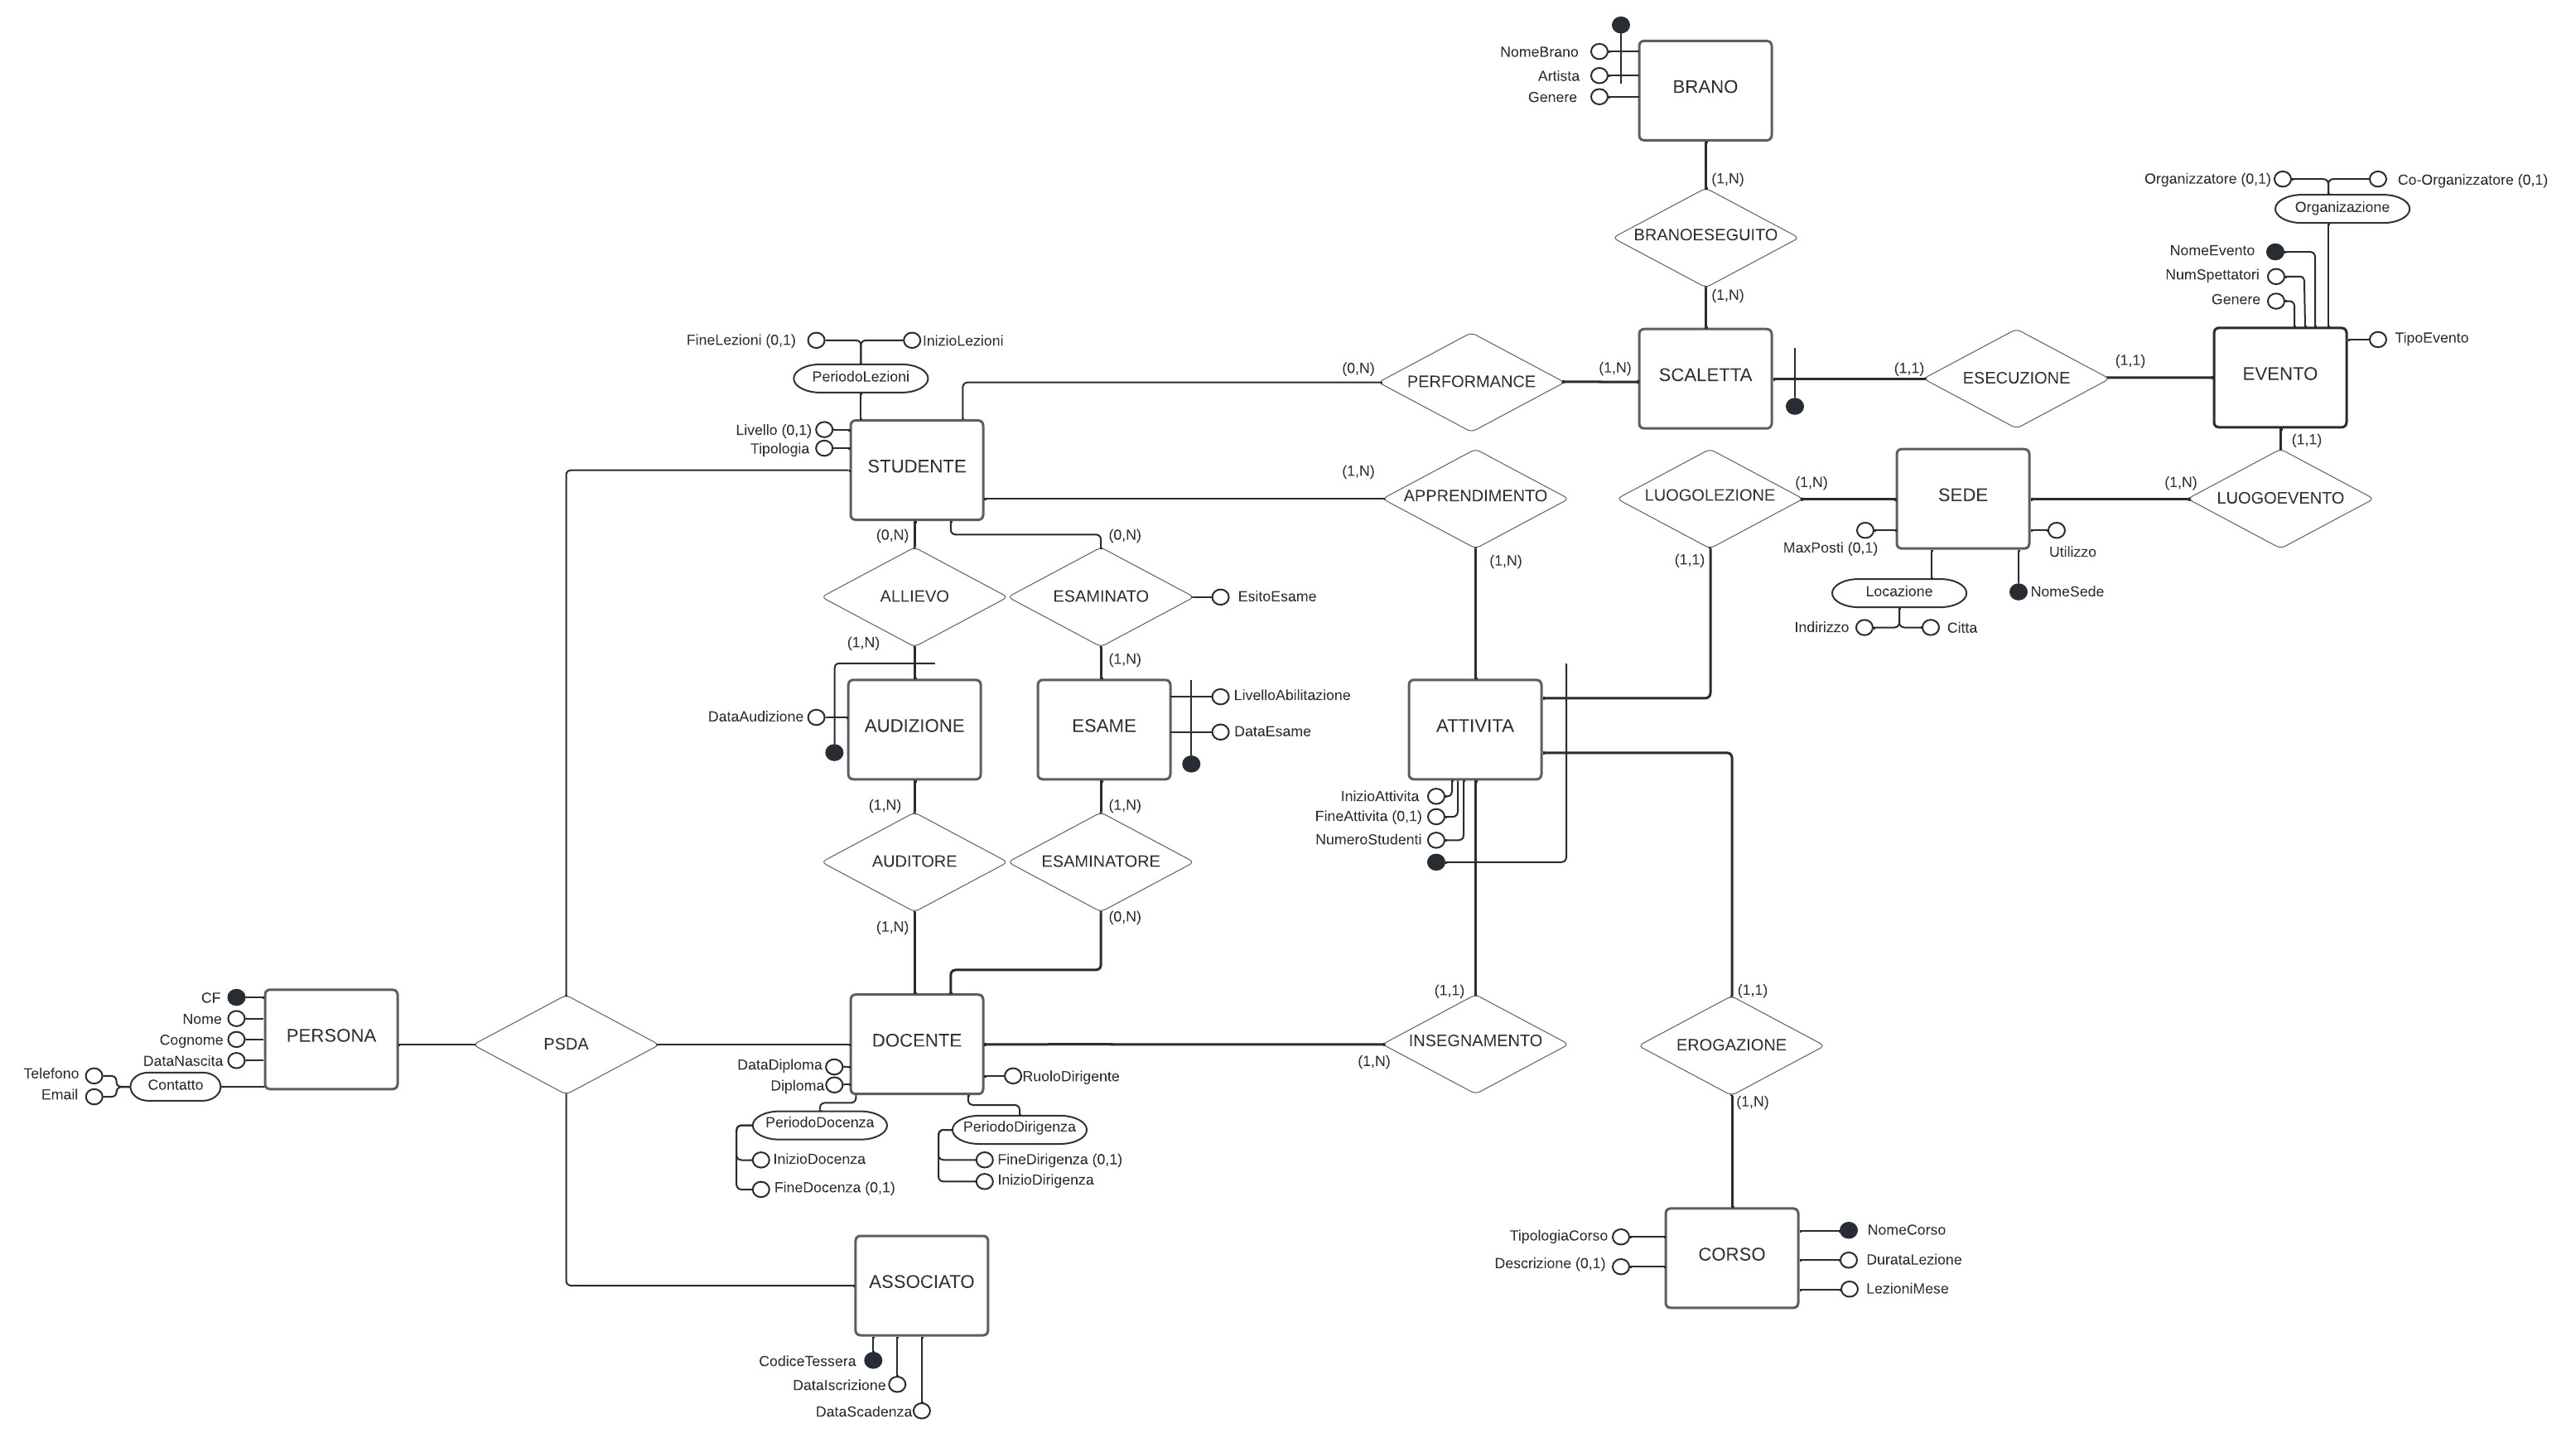
\includegraphics[scale=0.55]{../SchemaConcettuale/ER-LUCIDCHART - ER-concettuale 2.jpeg}
	\subsection{Schema relazionale e vincoli di integrità referenziale}
\section{Query}
\section{Indice}
\section{Codice C++}

\end{document}
